\documentclass[11pt,compress,t,notes=noshow, aspectratio=169, xcolor=table]{beamer}

\usepackage{../../style/lmu-lecture}
% Defines macros and environments
% This file is included in slides and exercises

% Rarely used fontstyle for R packages, used only in 
% - forests/slides-forests-benchmark.tex
% - exercises/single-exercises/methods_l_1.Rnw
% - slides/cart/attic/slides_extra_trees.Rnw
\newcommand{\pkg}[1]{{\fontseries{b}\selectfont #1}}

% Spacing helpers, used often (mostly in exercises for \dlz)
\newcommand{\lz}{\vspace{0.5cm}} % vertical space (used often in slides)
\newcommand{\dlz}{\vspace{1cm}}  % double vertical space (used often in exercises, never in slides)
\newcommand{\oneliner}[1] % Oneliner for important statements, used e.g. in iml, algods
{\begin{block}{}\begin{center}\begin{Large}#1\end{Large}\end{center}\end{block}}

% Don't know if this is used or needed, remove?
% textcolor that works in mathmode
% https://tex.stackexchange.com/a/261480
% Used e.g. in forests/slides-forests-bagging.tex
% [...] \textcolor{blue}{\tfrac{1}{M}\sum^M_{m} [...]
% \makeatletter
% \renewcommand*{\@textcolor}[3]{%
%   \protect\leavevmode
%   \begingroup
%     \color#1{#2}#3%
%   \endgroup
% }
% \makeatother


\title{Interpretable Machine Learning}
% \author{LMU}
%\institute{\href{https://compstat-lmu.github.io/lecture_iml/}{compstat-lmu.github.io/lecture\_iml}}
\date{}

\begin{document}

\newcommand{\titlefigure}{figure/pdp_bike}
\newcommand{\learninggoals}{
\item PD plots and relation to ICE plots
\item Interpretation of PDP
}

\lecturechapter{Partial Dependence (PD) plot}
\lecture{Interpretable Machine Learning}

\begin{frame}{Partial Dependence (PD) \citebutton{Friedman (2001)}{https://www.jstor.org/stable/2699986}}

\begin{columns}[T, totalwidth=\textwidth]
\begin{column}{0.55\textwidth}
\textbf{Definition:} PD function is expectation of $\fh(\xv_S, \xv_{-S})$ w.r.t. marginal distribution of features $\xv_{-S}$:
\begin{align*}
    f_{S, PD}(\xv_S) &= \E_{\xv_{-S}} \left( \fh(\xv_S, \xv_{-S}) \right) \\
    &= \int_{-\infty}^{\infty} \fh(\xv_S, \xv_{-S}) \, d\P(\xv_{-S})
\end{align*}

\medskip

\textbf{Estimation:} For a grid value $\xv_S^*$, average ICE curves point-wise at $\xv_S^*$ over all observed $\xv_{-S}^{(i)}$:
\begin{align*}
    \fh_{S, PD}(\xv_S^*) &= \frac{1}{n} \sum_{i=1}^n \fh(\xv_S^*, \xv_{-S}^{(i)})   \\
    &= \frac{1}{n} \sum_{i=1}^n \fhice{S}^{(i)}(\xv_S^*) 
\end{align*}

\end{column}

\begin{column}{0.43\textwidth}
\centering
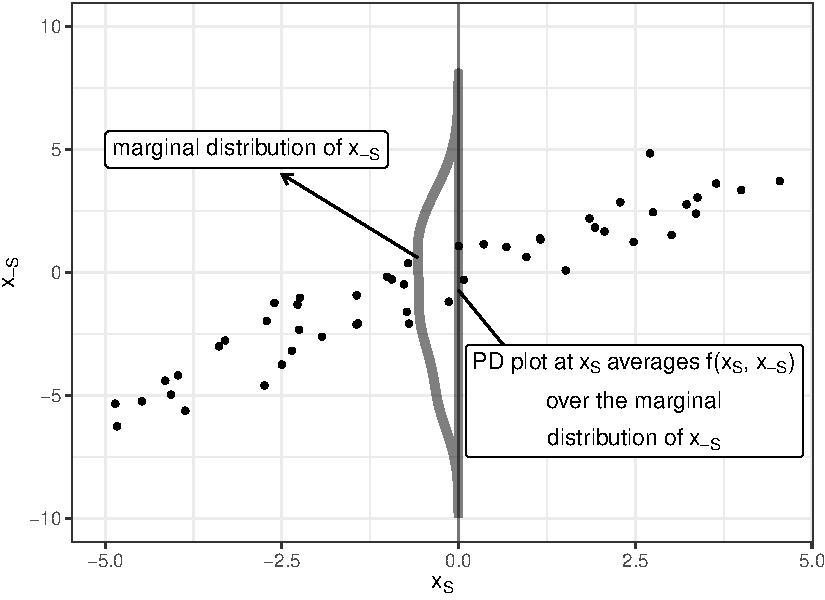
\includegraphics[width=\textwidth]{figure/pdplot.pdf}\\
\medskip
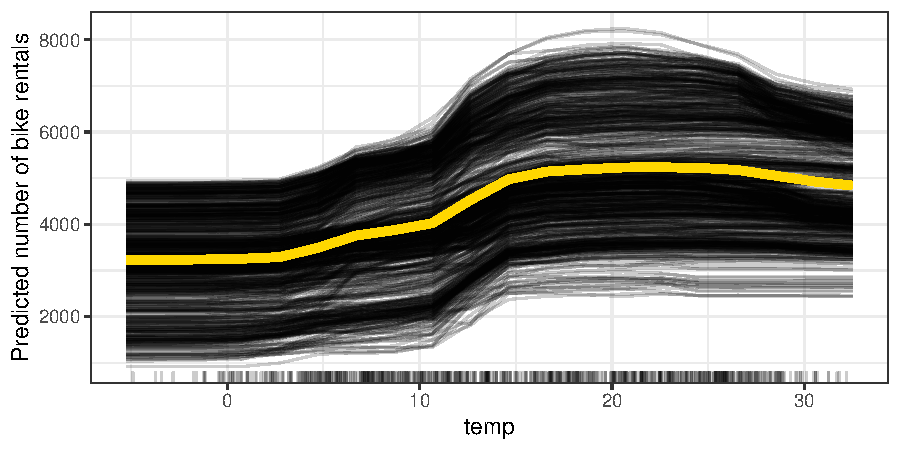
\includegraphics[width=\textwidth]{figure/pdp_bike.pdf}
\end{column}
\end{columns}
%Within the SIPA framework, the partial dependence builds the \textbf{Aggregation} step.

%\footnote[frame]{Friedman, Jerome H. (2001). Greedy Function Approximation: A Gradient Boosting Machine. Annals of Statistics: 1189-1232.}
%\footnote[frame]{Scholbeck, C. A., Molnar, C., Heumann, C., Bischl, B., and Casalicchio, G. (2019). Sampling, Intervention, Prediction, Aggregation: A Generalized Framework for Model Agnostic Interpretations. ECML PKDD 2019. (pp. 205-216).}
\end{frame}


\frame{
\frametitle{Partial Dependence}
%\begin{onlyenv}
\begin{columns}[T]
\begin{column}{0.5\textwidth}
\centering
\only<1>{
\includegraphics[page=8, width=0.8\textwidth]{../../figure_man/ice_pd_plot_demo}
\end{column}
\begin{column}{0.5\textwidth}

\begin{center}
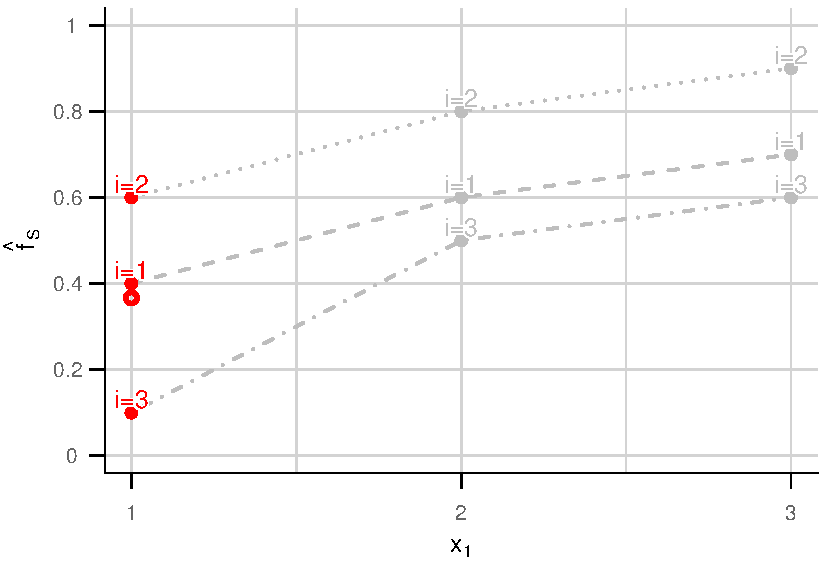
\includegraphics[page=1, width=\textwidth]{figure/PD}
\end{center}
}

\only<2>{
\includegraphics[page=9, width=0.8\textwidth]{../../figure_man/ice_pd_plot_demo}
\end{column}
\begin{column}{0.5\textwidth}

\begin{center}
\includegraphics[page=2, width=\textwidth]{figure/PD}
\end{center}
}

\only<3>{
\includegraphics[page=10, width=0.8\textwidth]{../../figure_man/ice_pd_plot_demo}
\end{column}
\begin{column}{0.5\textwidth}

\begin{center}
\includegraphics[page=3, width=\textwidth]{figure/PD}
\end{center}
}
\end{column}
\end{columns}
%\end{onlyenv}

Estimate PD function by \textbf{point-wise} average of ICE curves at grid value \fcolorbox{red}{white}{$\xv_S^* = x_1^* = \only<1>{1}\only<2>{2}\only<3>{3}$}:
$$\textstyle\fh_{1, PD}(x_1^*) = \frac{1}{n} \sum_{i=1}^n \fh(x_1^*, \xv_{2, 3}^{(i)})$$
}


\frame{
\frametitle{Example: PD for Linear Model}

Assume a linear regression model with two features:

$$\fh(\xv) = \fh(\xv_1, \xv_2) = \hat\theta_1 \xv_1 + \hat\theta_2 \xv_2 + \hat\theta_0$$

PD function for feature of interest $S = \{1\}$ (with $-S = \{2\}$) is:

$$
\begin{aligned}
f_{1, PD}(\xv_1) = \E_{\xv_2} \left( \fh(\xv_1, \xv_2) \right) &= \int_{-\infty}^{\infty} \left( \hat\theta_1 \xv_1 + \hat\theta_2 \xv_2 + \hat\theta_0 \right) \, d\P(\xv_2) \\
&= \hat\theta_1 \xv_1 + \hat\theta_2 \cdot \int_{-\infty}^{\infty} \xv_2 \, d\P(\xv_2) + \hat\theta_0 \\
&= \hat\theta_1 \xv_1 + \underbrace{\hat\theta_2 \cdot \E_{\xv_2} (\xv_2) + \hat\theta_0}_{:= const}
\end{aligned}
$$

$\Rightarrow$ PD plot visualizes the function $f_{1, PD}(\xv_1) = \hat\theta_1 \xv_1 + const$ ($\hat =$ feature effect of $\xv_1$).

}


\frame{
\frametitle{Interpretation: PD and ICE}

If feature varies:\\
\begin{itemize}
\item
  \textbf{ICE:} How does \textbf{prediction of
  individual observation} change? \(\Rightarrow\) \textbf{local} interpretation
\item
  \textbf{PD:} How does \textbf{average effect / expected prediction} change? \(\Rightarrow\) \textbf{global} interpretation
\end{itemize}

\begin{columns}[c]
\begin{column}{0.55\textwidth}
\begin{center}
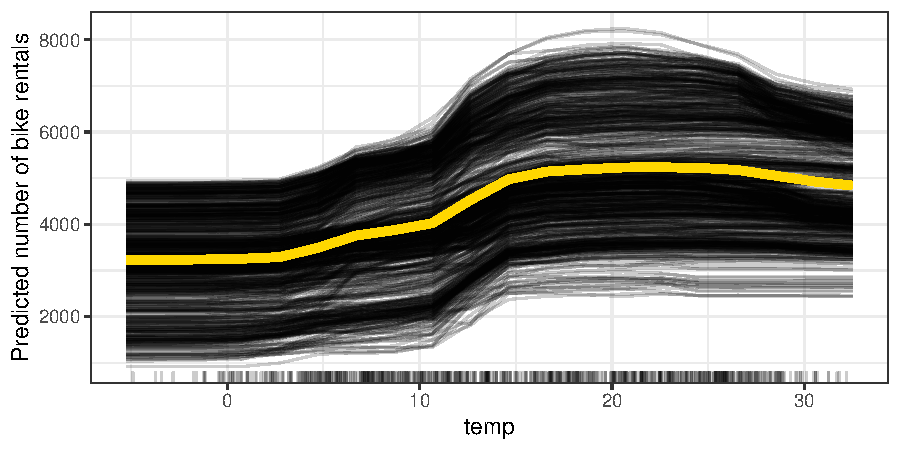
\includegraphics[width=\textwidth]{figure/pdp_bike}
\end{center}
\end{column}
\pause
\begin{column}{0.45\textwidth}
Insights from bike sharing data:
\begin{itemize}
%  \item Averaging ICE curves yields PD plot (yellow curve)
  \item Parallel ICE curves = homogeneous effect across observations
  \item Warmer $\Rightarrow$ more rented bikes
  \item Too hot $\Rightarrow$ slightly less bikes 
  \item The steepest increase in rentals occurs as temperature rises from 10°C to 15°C.
\end{itemize}
\end{column}
\end{columns}
}


\frame{
\frametitle{Interpretation: Categorical Features}

\begin{center}
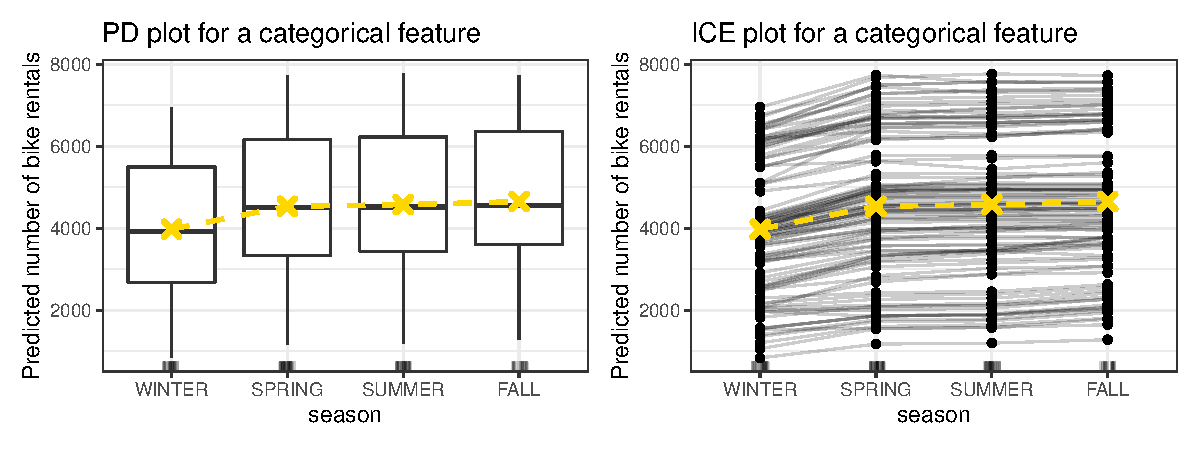
\includegraphics[width=0.9\textwidth]{figure/pdp_ice_cat}
\end{center}

\begin{itemize}
\item PDP with boxplots and ICE with parallel coordinates plots
%lot visualizes expected prediction if all observations would belong to a certain category (and shows distribution of predictions in a box plot)
\item NB: Categories can be unordered, if so, rather compare pairwise
\end{itemize}
%ICE plot connects predictions of individual observations (might identify heterogenous effects between categories if many lines are crossing)\\
%to identify heterogenous effects between categories (here: lines between SPRING and SUMMER are heterogenous).\\

}


% \begin{frame}{Comments on Extrapolation}

% % \begin{center}
% % \includegraphics[width=0.8\textwidth]{figure_man/extrapolation01.png}
% % \end{center}

% Extrapolation can cause issues in regions with few observations or if features are correlated
 
% \begin{columns}[T]
% \begin{column}{0.5\textwidth}
% \centering
% 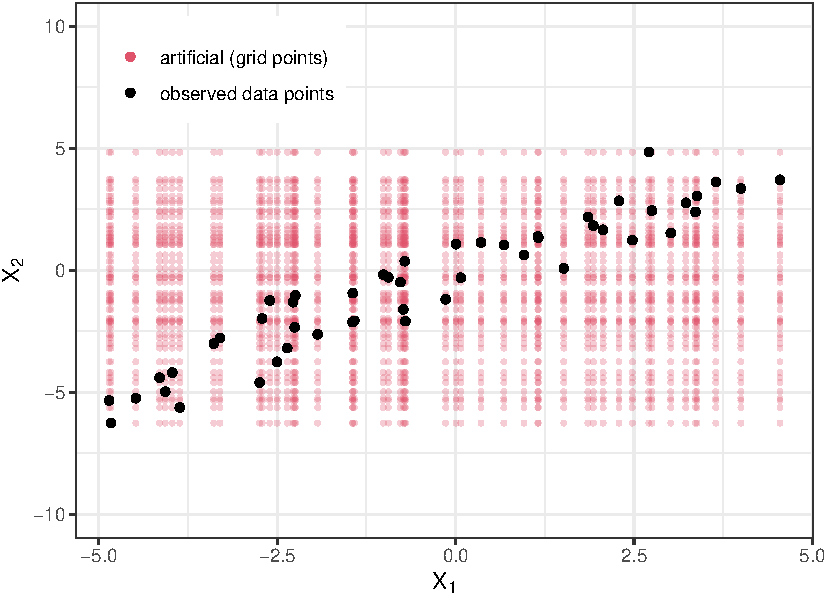
\includegraphics[width=0.8\textwidth]{figure/ale_scatter_grid}
% \end{column}
% \begin{column}{0.5\textwidth}
% \centering
% 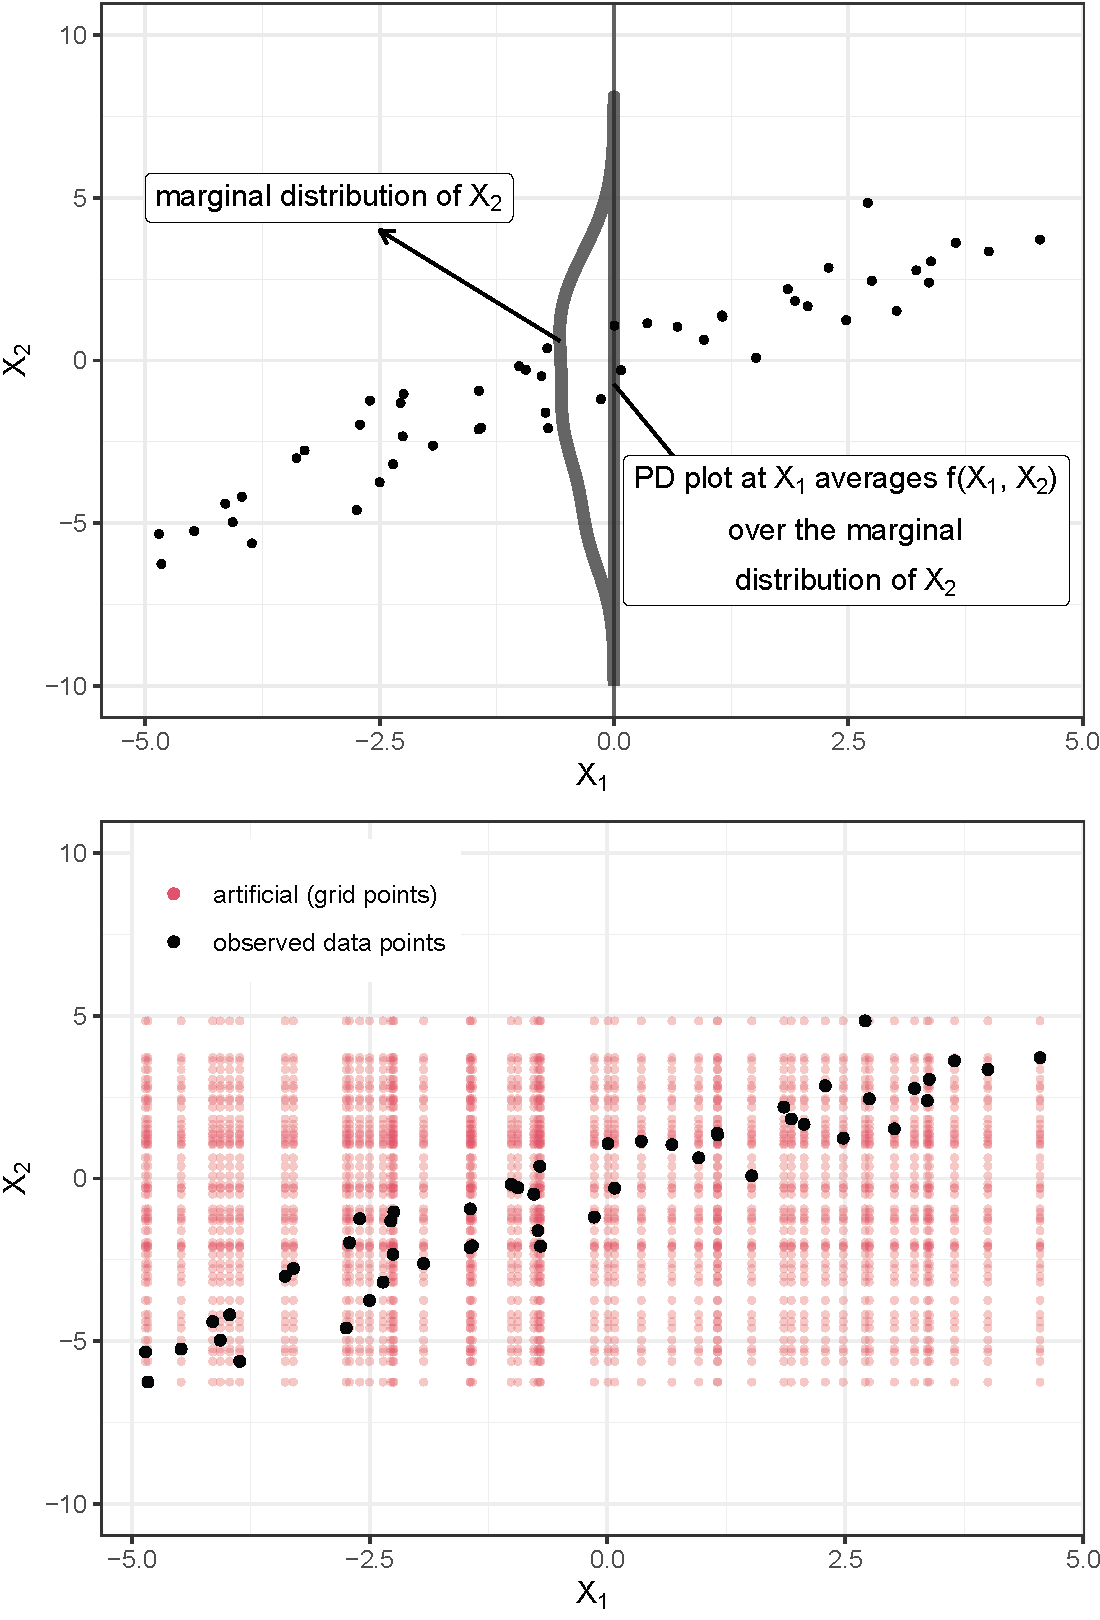
\includegraphics[width=0.8\textwidth]{figure/ale_pdplot}
% \end{column}
% \end{columns}

% \begin{itemize}
% \item \textbf{Example:} Features $x_1$ and $x_2$ are strongly correlated
% \item \textbf{Black points:} Observed points of the original data
% \item \textbf{\textcolor{red}{Red:}} Grid points used to calculate the ICE and PD curves (several unrealistic values)\\ %combination of feature values
% $\Rightarrow$ %Unrealistic combination of feature values are used, e.g., the
% PD plot at $x_1=0$ averages predictions over the whole marginal distribution of feature $x_2$\\
% $\Rightarrow$ May be problematic if model behaves strange outside training distribution
% %can bias ICE and PD curves Be careful with interpretations 
% %\item For correlated features and in regions with few observations with care
% %Extrapolation: interpret curves for highly correlated features and in feature regions with few observations with care
% \end{itemize}

% %
% % \framebreak
% %
% %
% % \begin{center}
% % \includegraphics[width=0.8\textwidth]{figure_man/extrapolation02.png}
% % \end{center}
% %
% % \begin{itemize}
% % \item The features $x_1$ and $x_2$ are strongly correlated.
% % \item \textcolor{red}{Red:} Observed points of the original data.
% % \item \textcolor{green}{Green:} Grid points used to calculate the ICE and PD curves.
% % \item Example: PD plot at $x_1=1.9$ averages predictions over the whole marginal distribution of feature $x_2$.
% % \end{itemize}
% \end{frame}




% % \begin{frame}{Interactions}
% %
% % For PD plots, the averaging of ICE curves might \textbf{obfuscate} heterogeneous effects and interactions. \newline \(\Rightarrow\) Ideally plot ICE curves and PD plots together.
% %
% % \begin{center}\includegraphics[width=0.65\textwidth]{figure_man/pdp_xor.pdf} \end{center}
% % %
% % % \framebreak
% % %
% % % \begin{itemize}
% % % \item
% % %   For PD plots, the averaging of ICE curves might \textbf{obfuscate}
% % %   heterogeneous effects and interactions. \newline \(\Rightarrow\)
% % %   Ideally plot ICE curves and PD plots together.
% % % \item
% % %   \textbf{Extrapolation:} Interprete curves for highly correlated
% % %   features and in feature regions with few observations with care.
% % % \item
% % %   Accumulated Local Effects (ALE) plots are a novel alternative to the PD plots developed by Apley (2020) that do not suffer from
% % %   extrapolation in case of correlated features.
% % % \end{itemize}
% % %
% % % \vspace{80pt}
% % % \tiny{
% % % Apley, D. W., \& Zhu, J. (2020). Visualizing the effects of predictor variables in black box supervised learning models. Journal of the Royal Statistical Society: Series B, 82(4), 1059-1086. \par}
% % \end{frame}

% \begin{frame}{Comments on Interactions}
% \begin{itemize}
% %\lz
% %\item Accumulated Local Effects (ALE) plots are a novel alternative to PD plots developed by Apley (2016) that do not suffer from extrapolation in case of correlated features.

% \item PD plots: averaging of ICE curves might \textbf{obfuscate} heterogeneous effects and interactions \\ 
% \(\Rightarrow\) Ideally plot ICE curves and PD plots together to uncover this fact\\
% \(\Rightarrow\) Different shapes of ICE curves suggest interaction (but does not tell with which  feature)

% \begin{center}\includegraphics[width=0.5\textwidth]{figure/pdp_xor.pdf} \end{center}
% \end{itemize}

% %\footnote[frame]{Apley, Daniel W., and Jingyu Zhu (2020). Visualizing the Effects of Predictor Variables in Black Box Supervised Learning Models. Journal of the Royal Statistical Society: Series B (Statistical Methodology) 82.4: 1059-1086.}
% \end{frame}

% \begin{frame}{Comments on Interactions - 2D Partial Dependence}

% \begin{center}
% 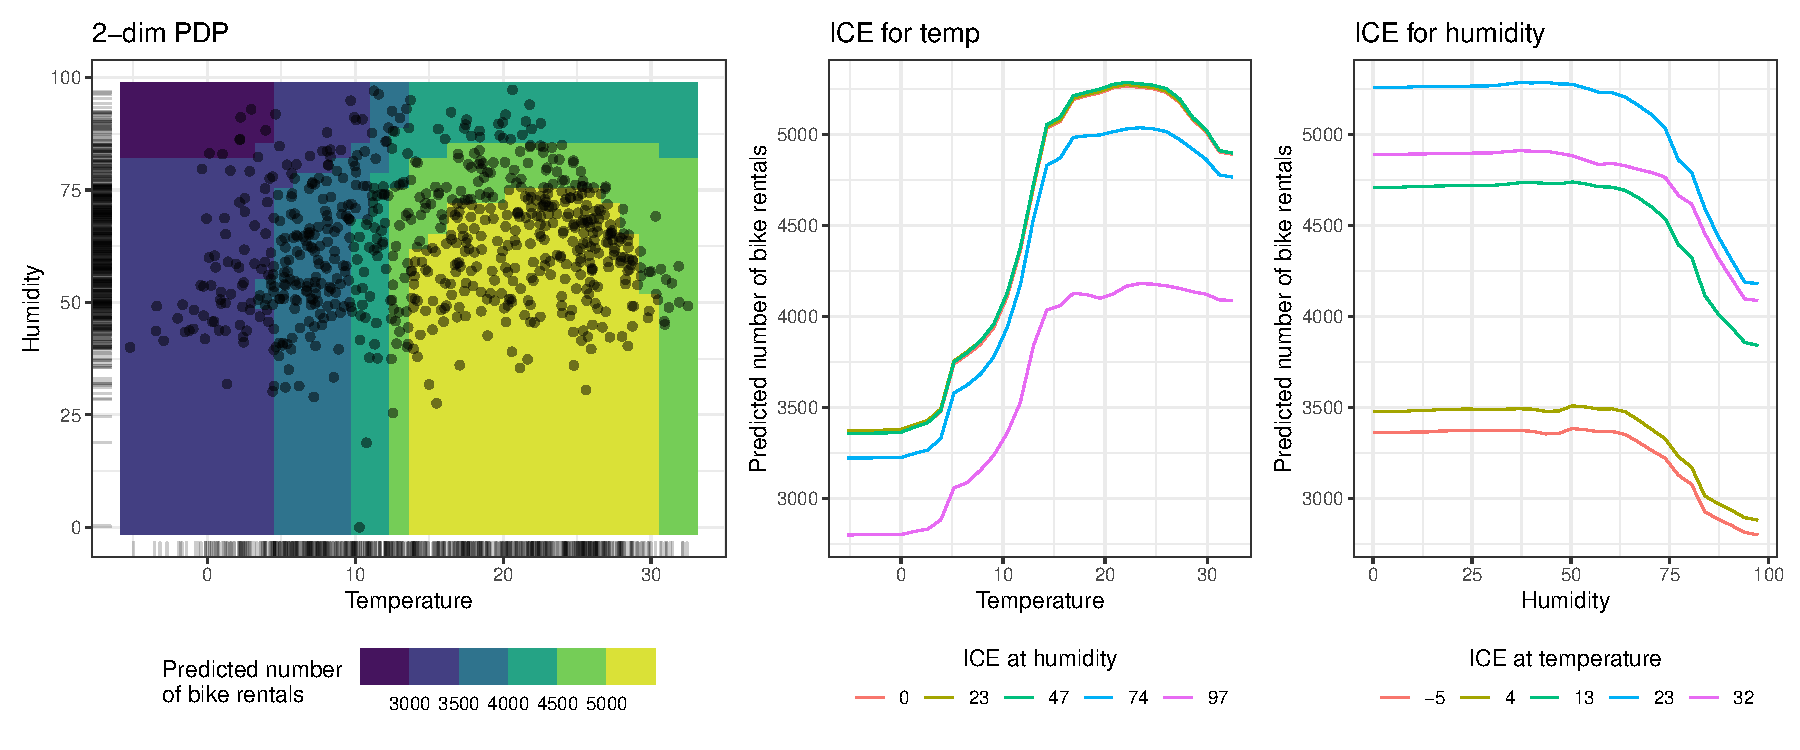
\includegraphics[width=0.9\textwidth]{figure/pdp2d_bike}
% \end{center}

% \begin{itemize}
%  \item Humidity and temperature interact with each other at high values (see shape difference)\\
%  $\leadsto$ Shape of ICE curves at different horizontal and vertical slices varies (for high values)
%  \item Low to medium humidity and high temperature $\Rightarrow$ many rented bikes
%  %Many rented bikesThe number of bike rentals is especially high when humidity is below 75 percent and temperature is between 15 $^{\circ}$C and 27 $^{\circ}$C
% \end{itemize}


% % \framebreak
% %
% % add datapoints to previous figure and mention convex hull (see pdp package)

% \end{frame}


% \begin{frame}{Centered ICE Plot (c-ICE)}

% \textbf{Issue:} Difficult to identify heterogenous ICE curves if curves have different intercepts (are stacked)
% %When ICE curves start at different intercepts (are stacked), it is difficult to identify heterogenous predictions.

% \textbf{Solution:} Center ICE curves at fixed reference value $x' \sim \P(\xv_S)$, often $x' = \min(\xv_S)$\\
% $\Rightarrow$ Easier to identify heterogenous shapes with c-ICE curves
% \vspace{-0.2cm}
% \begin{columns}[c]
% \begin{column}{0.45\textwidth}
% %\centering
% $$\begin{aligned}
% \fh_{S, cICE}^{(i)}(\xv_S)
% &= \fh(\xv_S, \xi_{-S}) - \fh(x', \xi_{-S}) \\
% &= \fh_{S}^{(i)}(\xv_S) - \fh_{S}^{(i)}(x')
% \end{aligned}$$

% $\Rightarrow$ Visualize $\fh_{S, cICE}^{(i)}(\xv_S^*)$ vs. $\xv_S^*$

% \lz
% \pause
% \textbf{Interpretation} (yellow curve in c-ICE): \\
% On average, the number of bike rentals at $\sim 97$ \% humidity decreased by 1000 bikes compared to a humidity of 0 \%
% \end{column}
% \begin{column}{0.54\textwidth}
% \begin{center}
% %\vspace{-0.3cm}
% 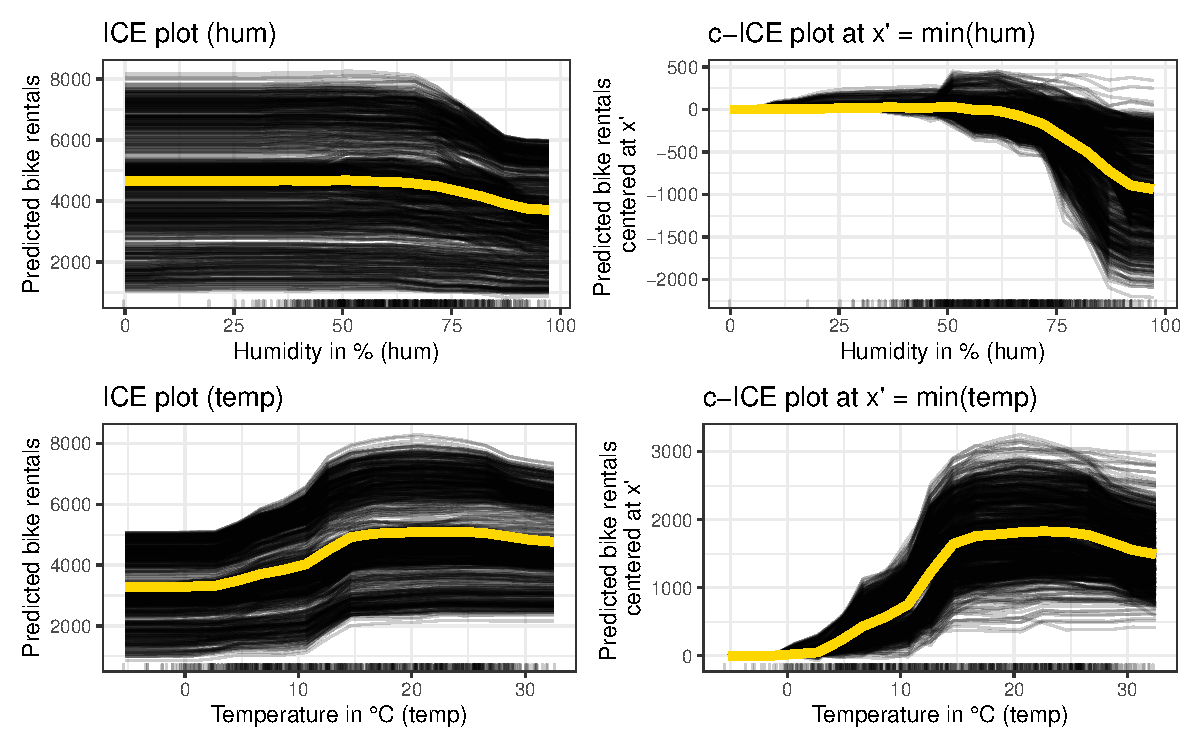
\includegraphics[width=\textwidth]{figure/cICE}
% \end{center}
% \end{column}
% \end{columns}

% %\vspace{-0.4cm}

% \end{frame}


% \begin{frame}{Centered ICE Plot (c-ICE)}

% For categorical features, c-ICE plots can be interpreted as in LMs due to reference value

% \begin{columns}[c]
% \begin{column}{0.44\textwidth}

% \begin{center}
% 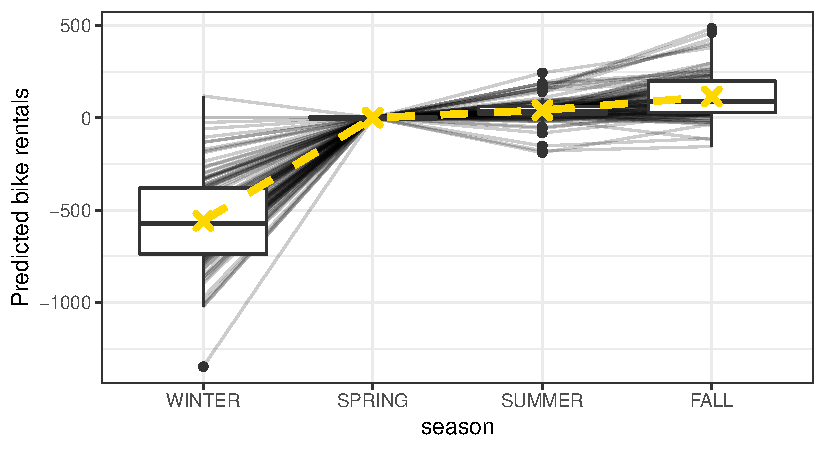
\includegraphics[width=\textwidth]{figure/cICEcat}
% \end{center}

% \end{column}
% \begin{column}{0.55\textwidth}

% \textbf{Interpretation}: \\
% \begin{itemize}
% %\item Centered ICE plots are useful for categorical features and can be interpreted as in LMs
% \item The reference category is $x' =$ SPRING
% \item Golden crosses: Average number of bike rentals if we jump from SPRING to any other season\\
% $\Rightarrow$ Number of bike rentals drops by $\sim 560$ in \code{WINTER} and is slightly higher in \code{SUMMER} and \code{FALL} compared to \code{SPRING}
% \end{itemize}

% \end{column}
% \end{columns}

% \end{frame}


\endlecture
\end{document}
